\section{Содержание работы}

\subsection{Основные сведения}

Триод является вакуумным электронным прибором, отличающимся от диода наличием
третьего электрода, расположенного между катодом и анодом и называемого
управляющей сеткой или просто сеткой.

На рисунке~\pic{1} показаны распространенные конструкции электродов триода.
\begin{figure}[ht]
  \center
  \includegraphics[width=.4\textwidth]{1_1} \hspace{2em}
  \includegraphics[width=.4\textwidth]{1_2}
  \caption{Конструкция электродов триода}
  \label{pic1}
\end{figure}

Действие управляющей сетки заключается в том, что она регулирует распределение
пространственного заряда между катодом и анодом и, таким образом, управляет
потоком электронов внутри лампы, то есть анодным током. Вследствие того, что
сетка не является сплошной, она свободно пропускает электроны, летящие к аноду.
С другой стороны, она формирует структуру поля, причем резко ослабляется
влияние изменения анодного напряжения на поле вблизи катода --- экранирует
катод от анода и ослабляет действие анода на электроны, вылетающие с катода.

Напряжением на сетке или сеточным напряжением называют разность потенциалов
между сеткой и катодом, то есть потенциал сетки относительно катода. В лампах
с катодом прямого накала все напряжения отсчитывают относительного
отрицательного конца катода.

На рисунке \pic{2} показано распределение поля в триоде при различных
величинах напряжения на сетке и фиксированном анодном напряжении. Видно, что
сетка задерживает большую часть поля. Чем гуще сетка, тем сильнее экранирует
она катод от влияния анода. Вследствие этого и отчасти потому, что сетка
расположена ближе к катоду, чем к аноду, небольшие изменения потенциала на
сетке оказывают гораздо более сильное действие на анодный ток, чем значительные
изменения потенциала на аноде.

\begin{figure}[ht]
  \center
  \includegraphics[width=.9\textwidth]{2}
  \caption{Распределение электростатического потенциала плоского триода при
  различных потенциалах сетки и одинаковом анодном напряжении}
  \label{pic2}
\end{figure}

При небольшом отрицательном напряжении сетка отталкивает электроны, но часть их
все же пролетает в ее просветы благодаря притяжению анода. Однако можно
увеличить отрицательное напряжение настолько, что она будет отталкивать все
электроны и анодный ток прекратится. Лампа будет заперта.

В этом случае условие прекращение анодного тока соответствует равенству
\begin{equation}
  U_C = -DU_A,
  \label{eq2}
\end{equation}
где \( D \)~-- проницаемость сетки, пропорциональная отношению диаметра сетки
к периоду ее намотки, \( U_C \)~-- напряжение на сетке, \( U_A \)~-- напряжение на
аноде.

При увеличении напряжения на сетке (но при условии, что \( U_C < 0 \)) анодный
ток совпадает по величине с катодным и растет по закону Ленгмюра \eqref{eq1}.

В результате характер изменения анодного тока в триоде может быть описан двумя
характеристиками: анодно-сеточной, когда при фиксированном анодном напряжении
изменяется напряжение на сетке (рис.~\pic{3}), и анодной, когда
напряжение на сетке остается постоянным, но варьируется величина напряжения на
аноде (рис.~\pic{4}). Обе характеристики взаимосвязаны~--- и по семейству
анодно-сеточных характеристик легко построить анодную.

\begin{figure}[ht]
  \center
  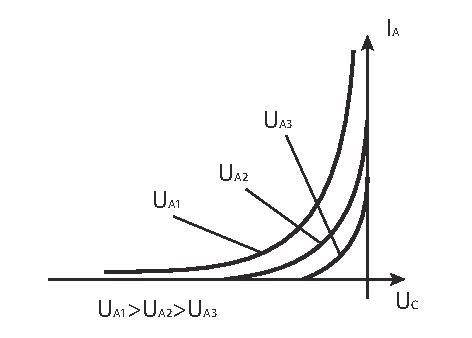
\includegraphics[width=.45\textwidth]{3} \hspace{2em}
  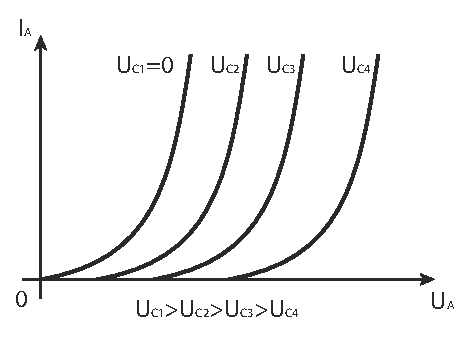
\includegraphics[width=.45\textwidth]{4}
  \parbox{.45\textwidth}{\caption{Семейство анодно-сеточных характеристик
  триода}\label{pic3}} \hspace{2em}
  \parbox{.45\textwidth}{\caption{Семейство анодных характеристик триода}
  \label{pic4}}
\end{figure}

\subsection{Электроника триода}

В общем случае анализ электроники триода основан на формуле для действующего
потенциала сетки:
\begin{equation}
  U_D = \sigma (U_C + D U_A),
  \label{eqel}
\end{equation}
где \( \sigma \)~-- параметр, который носит название остроты управления и
равный приблизительно величине \( \sigma \approx 1/(1 + D) \).

Прохождение анодного тока через триод можно описать, введя представление
эквивалентного диода, то есть такого диода, у которого плоскость анода
совпадает с плоскостью сетки в триоде. В этом случае катодный ток подчиняется
классическому закону Ленгмюра:
\begin{equation}
  I_k = P(U_C + DU_A)^{3/2},
  \label{eq1}
\end{equation}
где  \( P \)~-- первеанс триода, зависящий от геометрических
размеров триод.

Введем коэффициент токопрохождения \( s = I_a/I_k \) и коэффициент
токораспределения \( k = I_a/I_c \). Оба эти коэффициента равнозначны, но чаще
используют коэффициент \( s \), зная который легко определяются величины всех
токов:
\[
  I_a = s I_k; \qquad I_c = (1 - s) I_k; \qquad \frac{s}{k} = 1 - s.
\]

Выделяют два режима работы триода:
\vspace{-.5em}
\begin{itemize}
  \itemsep -.5pt
  \item режим токоперехвата (при \( U_A > U_D \));
  \item режим возврата электронов (при \( U_A < U_D \)).
\end{itemize}

\subsubsection{Режим токоперехвата}

В данном режиме ток сетки будет определяться только теми электронами, которые
будут перехватываться сеткой при их непосредственном движении от катода к аноду.

\begin{figure}[h!]
  \center
  \includegraphics[width=.6\textwidth]{cur_catch}\\
  \vspace{-1em}\parbox{1em}{\small а)}\hspace{8em}\parbox{1em}{\small б)}
  \caption{Режим токоперехвата}
  \label{picCC}
\end{figure}

Предположим, что эмиссия электронов с катода равномерна и прямолинейна.
Тогда коэффициент токопрохождения будет определяться отношением площади катода, не
находящейся под поверхностью сетки, к полной площади катода (рис.~\pic{CC}а):
\begin{equation}
  s_0 = \frac{L_\text{не под сеткой}}{L} = \frac{L - 2 R_c}{L} =
    1 - \frac{2 R_c}{L}.
  \label{eqs0}
\end{equation}

В зависимости от знака напряжения на сетке \( U_C \) может наблюдаться
два случая: при \( U_C < 0 \) коэффициент токопрохождения \( s \) будет больше
\( s_0 \), а при \( U_C > 0 \)~-- меньше \( s_0 \).

Рассмотрим второй случай.

Пускай электрон вылетает на некотором расстоянии \( R_\text{эф} \) от центра
элемента сетки (рис.~\pic{CC}б).

По закону сохранения момента импульса (при нулевой начальной скорости
электрона):
\[
  m v_d R_\text{эф} = m v_c R_c.
\]

Выразим скорости из закона сохранения энергии:
\[
  \frac{m v_d^2}{2} = e U_D, \quad \frac{m v_c^2}{2} = e U_C; \quad \Rightarrow
    \quad v_d = \sqrt{\frac{2 e}{m} U_D}, \quad v_c = \sqrt{\frac{2 e}{m} U_C}.
\]

Тогда \( R_\text{эф} = R_c \cdot \sqrt{U_C / U_D} \). Подставляя в \eqref{eqs0}
\( R_\text{эф} \) вместо \( R_c \), получим
\begin{equation}
  s = 1 - \frac{2 R_\text{эф}}{L} = 1 - \frac{2 R_c}{L} \sqrt{\frac{U_C}{U_D}}.
  \label{eqdntt}
\end{equation}

Из формулы~\eqref{eqel} следует, что \( U_C = U_D / \sigma - D U_A \); подставим
в~\eqref{eqdntt}:
\[
  s = 1 - \frac{2 R_c}{L} \sqrt{\frac{U_D}{\sigma U_D} - \frac{D U_A}{U_D}} =
    1 - \frac{2 R_c}{L} \sqrt{\frac{1}{\sigma} - D \frac{U_A}{U_D}}.
\]

\subsubsection{Режим возврата электронов}

Режим возврата электронов возникает, когда между сеткой и анодом действует
тормозящее поле, возвращающее часть электронов обратно к сетке.

Представим траекторию электрона в виде ломаной кривой (рис.~\pic{EB}).
\begin{figure}[h!]
  \center
  \includegraphics[width=.6\textwidth]{els_back}
  \caption{Режим возврата электронов}
  \label{picEB}  
\end{figure}

У крайнего электрона перпендикулярная аноду составляющая скорости равна нулю,
пройдя область сетки он вылетает под углом \( \alpha_\text{кр} \):
\[
  e (U_D - U_A) = \frac{m (v_d \cos\alpha_\text{кр})^2}{2}.
\]
Так как \( e U_D = m v_d^2 / 2 \), то
\( \sin\alpha_\text{кр} = \sqrt{U_A / U_D} \).

Анода будут достигать те электроны, которые вылетают под углом
\( \alpha < \alpha_\text{кр} \).

Действие сетки на электрон аналогично действию рассеивающей линзы-диафрагмы,
оптическая сила которой:
\[
  \frac{1}{f} = \frac{1}{4 \sqrt{U_0}} \int\lii \frac{U_0''}{\sqrt{U_0}}\,dz.
\]

Считая, что \( U_0'' \ne 0 \) только при \( z = 0 \), то \( U_0 = U_D \) и
\[
  \frac{1}{f} = \frac{1}{4 U_D} \int\lii U_0''\,dz = \frac{1}{4 U_D} \left(
    \frac{U_A - U_D}{d_\text{са}} - \frac{U_D}{d_\text{кс}} \right).
\]

Тогда фокусное расстояние:
\[
  f = 4 U_D \frac{d_\text{са} d_\text{кс}}{d_\text{кс} (U_A - U_D) -
    d_\text{са} U_D} = 4 U_D \frac{d_\text{са} d_\text{кс}}
    {d_\text{кс} U_A - d_\text{ка} U_D},
\]
где \( d_\text{ка} = d_\text{кс} + d_\text{са} \)~-- расстояние от катода до
анода.

Так как \( d_\text{кс} \ll d_\text{ка} \), то
\[
  f \approx -4 U_D \frac{d_\text{са} d_\text{кс}}{d_\text{ка} U_D} = 
    -4 \frac{d_\text{са} d_\text{кс}}{d_\text{ка}}.
\]

Тогда \( \tg\alpha_\text{кр} = y_\text{кр} / f \), а так как
\( \alpha_\text{кр} \) мало, то \( \tg\alpha_\text{кр} \sim
\sin\alpha_\text{кр} \).

Получаем, что
\[
  y_\text{кр} = f \sin\alpha_\text{кр} = f \sqrt{\frac{U_A}{U_D}} =
    4 \frac{d_\text{са} d_\text{кс}}{d_\text{ка}} \sqrt{\frac{U_A}{U_D}}.
\]

Таким образом, коэффициент токопрохождения, аналогично \eqref{eqs0}:
\[
  s = \frac{I_a}{I_k} = \frac{2 y_\text{кр}}{L} =
    4 \frac{d_\text{са} d_\text{кс}}{d_\text{ка} L} \sqrt{\frac{U_A}{U_D}}.
\]

На рисунке \pic{5} приведена типичная кривая токораспределения (без учета
начальных скоростей электронов и полей пространственного заряда).

\begin{figure}[!b]
  \center
  \includegraphics[width=.7\textwidth]{5}
  \caption{Кривая токораспределения в плоском триоде\\
  I~-- область возврата электронов; II~-- область токоперехвата}
  \label{pic5}
\end{figure}

\section{Описание экспериментальной установки}

На рисунке~\pic{Look} приведен внешний вид экспериментальной установки по
изучению статических характеристик триода.

\begin{figure}[ht]
  \center
  \includegraphics[width=.5\textwidth]{photo}
    \caption{Внешний вид экспериментальной установки} \label{picLook}
  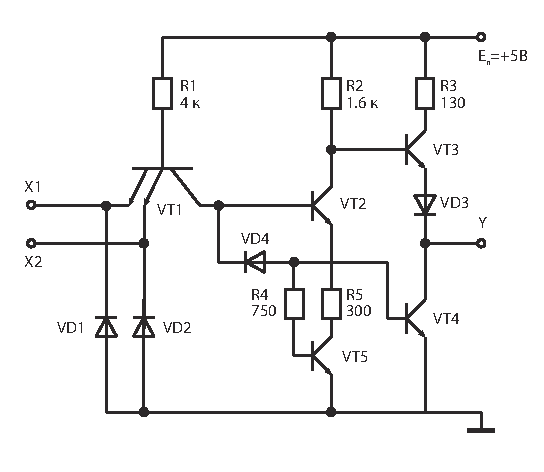
\includegraphics[width=.8\textwidth]{scheme}
    \caption{Принципиальная электрическая схема установки} \label{picScheme}
\end{figure}

\begin{enumerate}
  \item Вольтметр.
  \item Амперметр.
  \item Регулятор сеточного напряжения.
  \item Регулятор анодного напряжения.
  \item Переключатель измеряемого напряжения.
  \item Выключатель сетевого напряжения.
\end{enumerate}

Принципиальная схема экспериментальной установки представлена на
рисунке~\pic{Scheme}.

\section{Методика проведения эксперимента}
\renewcommand{\labelenumi}{4.\arabic{enumi}.}
\begin{enumerate}
  \item Включив сеть, дать прибору прогреться не менее 3~мин.
  \item Переключатель~5 должен находиться в положении <<\( U_A \)>>, а
    регулятор~3 должен быть повернут вправо до упора.
  \item Подать на анод максимально возможное напряжение регулятором~4
    (\( U_{a_m} \sim \)40~В). Зафиксировать значение анодного тока.
  \item Переключив тумблер~5 в положение <<\( U_C \)>>, повысить по модулю
    напряжение на сетке на одно деление регулятором~3. Переключить~5 в положение
    <<\( U_A \)>> и регулятором~4 вернуть напряжение на аноде к \( U_{a_m} \).
    Записать значение анодного тока.
  \item Повторяя пункт~4 для различных \( U_{a_m} \), снять зависимость
    \( I_a(U_c) \) при \( U_a = \const \). Данные занести в
    таблицу~\ref{grid-anod}.

    \begin{table}[ht]
      \center
      \caption{Семейство анодно-сеточных характеристик}
      \label{grid-anod}
      \begin{tabular}{|m{.1\textwidth}|C{.12}|*{7}{C{.07}|}} \hline
        \multirow{5}{*}{\( U_{a_{01}} \)} &
          \( U_c \),~В &&&&&&& \\ \cline{2-9}
        & \( I_{a_1} \),~мА &&&&&&& \\ \cline{2-9}
        & \( I_{a_2} \),~мА &&&&&&& \\ \cline{2-9}
        & \( I_{a_3} \),~мА &&&&&&& \\ \cline{2-9}
        & \( \average{I_a} \),~мА &&&&&&& \\ \hline
        \multirow{4}{*}{\( U_{a_{02}} \)} &
          \( U_c \),~В &&&&&&& \\ \cline{2-9}
        \multirow{4}{*}{и т.~д.} &
          \( I_{a_1} \),~мА &&&&&&& \\ \cline{2-9}
        & \( I_{a_2} \),~мА &&&&&&& \\ \cline{2-9}
        & \( I_{a_3} \),~мА &&&&&&& \\ \cline{2-9}
        & \( \average{I_a} \),~мА &&&&&&& \\ \hline
      \end{tabular}
    \end{table}

  \item Зафиксировав напряжение на сетке регулятором~3, изменять напряжение на
    аноде регулятором~4 и снять зависимость \( I_a(U_a) \) при
    \( U_c = \const \).
  \item Повторить пункт~6 для различных напряжениях на сетке\\
    \( U_c = \const \). Результаты занести в таблицу~\ref{anod-anod}.
    
    \begin{table}[ht]
      \center
      \caption{Семейство анодных характеристик триода}
      \label{anod-anod}
      \begin{tabular}{|m{.1\textwidth}|C{.12}|*{7}{C{.07}|}} \hline
        \multirow{5}{*}{\( U_{c_{01}} \)} &
          \( U_a \),~В &&&&&&& \\ \cline{2-9}
        & \( I_{a_1} \),~мА &&&&&&& \\ \cline{2-9}
        & \( I_{a_2} \),~мА &&&&&&& \\ \cline{2-9}
        & \( I_{a_3} \),~мА &&&&&&& \\ \cline{2-9}
        & \( \average{I_a} \),~мА &&&&&&& \\ \hline
        \multirow{4}{*}{\( U_{c_{02}} \)} &
          \( U_a \),~В &&&&&&& \\ \cline{2-9}
        \multirow{4}{*}{и т.~д.} &
          \( I_{a_1} \),~мА &&&&&&& \\ \cline{2-9}
        & \( I_{a_2} \),~мА &&&&&&& \\ \cline{2-9}
        & \( I_{a_3} \),~мА &&&&&&& \\ \cline{2-9}
        & \( \average{I_a} \),~мА &&&&&&& \\ \hline
      \end{tabular}
    \end{table}
    
    \item Построить графики анодно-сеточной и анодной характеристик на
      миллиметровой бумаге.
    \item По экспериментально определенным анодно-сеточным характеристикам
      построить семейство анодных характеристик и сравнить с анодными
      характеристиками, полученными экспериментально.
\end{enumerate}